\documentclass[%
autoref,     % тип документа
href,        % использовать пакет hyperref для создания гиперссылок
facsimile,   % отображать факсимиле диссертанта и ученого секретаря
colorlinks,  % цветные гиперссылки
%fixint,     % отключить прямые знаки интегралов
%times,      % шрифт Times как основной
%classified, % гриф секретности
]{disser}

\usepackage[
  a4paper, mag=1000,
  left=2.5cm, right=1cm, top=2cm, bottom=2cm, headsep=0.7cm, footskip=1cm
]{geometry}
\usepackage{amsmath, amsthm, amssymb}
\usepackage[T1,T2A]{fontenc}
\usepackage[utf8]{inputenc}
\usepackage[english,russian]{babel}
\usepackage{tabularx}
\usepackage{csquotes}
\ifpdf\usepackage{epstopdf}\fi
\usepackage{lastpage}

\usepackage[style=gost-numeric,
  backend=biber,
  language=auto,
  hyperref=auto,
  autolang=other,
  defernumbers=true,
  maxbibnames=4,
  sorting=none,
  movenames=false
]{biblatex}

\addbibresource{thesis.bib}

% Номера страниц снизу и по центру
\pagestyle{footcenter}
\chapterpagestyle{footcenter}

% Точка с запятой в качестве разделителя между номерами цитирований
%\setcitestyle{semicolon}

% Путь к файлам с иллюстрациями
\graphicspath{{fig/}}

\newtheorem{theorem}{Теорема} 
\newtheorem{cor}{Следствие} 
\newtheorem{lemma}{Лемма}
\newtheorem{fact}{Утверждение}
\newtheorem{remark}{Замечание}

\begin{document}
% Включение файла с общим текстом диссертации и автореферата
% (текст титульного листа и характеристика работы).
% Общие поля титульного листа диссертации и автореферата
\institution{Название организации}

\topic{Тема диссертации}

\author{Скурыдина Алия Фиргатовна}

\specnum{01.01.07}
\spec{Вычислительная математика}
%\specsndnum{01.04.07}
%\specsnd{Физика конденсированного состояния}

\sa{Акимова Елена Николаевна}
\sastatus{д.~ф.-м.~н., доц.}
%\sasnd{ФИО второго руководителя}
%\sasndstatus{к.~ф.-м.~н., проф.}

%\scon{ФИО консультанта}
%\sconstatus{д.~ф.-м.~н., проф.}
%\sconsnd{ФИО второго консультанта}
%\sconsndstatus{д.~ф.-м.~н., проф.}

\city{Екатеринбург}
\date{\number\year}

% Общие разделы автореферата и диссертации
\mkcommonsect{actuality}{Актуальность темы исследования.}{%
Построение итеративно регуляризованных алгоритмов востребовано для решения широкого круга прикладных некорректно поставленных задач. Так, решение структурных обратных задач гравиметрии и магнитометрии сводится к решению нелинейных интегральных уравнений Урысона первого рода. После дискретизации операторное уравнение сводится к системе нелинейных уравнений с большим числом неизвестных, поэтому есть необходимость в параллелизации алгоритмов для многопроцессорных и многоядерных вычислительных систем с целью уменьшения времени счета. 
}

\mkcommonsect{development}{Степень разработанности темы исследования.}{
Ж. Адамар в 1902 г.~\cite{Hadamar1902} впервые определил условия корректности задачи математической физики. Задачи, не отвечающие этим условиям, то есть некорректные,  Ж. Адамар считал лишенными физического смысла. В течение многих лет обратные задачи решались методом подбора, например, в геофизике, сравнивая вычисленное физическое поле модели с наблюденным. Однако со временем, это мнение претерпело изменения.

Первой работой по теории некорректных задач считается известная работа академика А.Н. Тихонова 1943 г.~\cite{Tikh1943}, в которой он доказал устойчивость некоторых обратных задач при условии принадлежности решения компактному множеству. Также в этой работе он решил одну из актуальных обратных задач разведочной геофизики. В дальнейшем теория некорректных задач оформилась в самостоятельный раздел современной математики. В конце 50-х годов и начале 60-х годов появились работы, посвященные решению некоторых некорректных задач с помощью идей регуляризации, выдающихся отечественных ученых: А.Н. Тихонова, М.М. Лаврентьева, В.К. Иванова. Их исследования в этой области положили начало трем научным школам:  Московской, Сибирской и Уральской.
Началось исследование устойчивых методов решения некорректно-поставленных задач, представляющих собой одно из наиболее актуальных проблем современной математической науки.

В большом цикле работ, выполненных начиная с 1963 года, А.Н. Тихонов сформулировал принцип устойчивого решения некорректно-поставленных задач, ввел понятие регуляризирующего оператора и предложил ряд эффективных методов построения таких операторов, легко реализуемых на ЭВМ ~\cite{Tikh1963_1, Tikh1963_2, TikhGlas1965, TikhArs1986}. Метод, получивший название "метод регуляризации А.Н. Тихонова"\, был применен для решения большого количества как фундаментальных математических, так и актуальных прикладных задач. В частности, тихоновским методом регуляризации были решены задача об отыскании решения интегрального и операторного уравнения первого рода, обратные задачи теории потенциала и теплопроводности. 

Наряду с Тихоновым, М.М. Лаврентьев изучал методы регуляризации. Ему принадлежит идея замены исходного уравнения близким ему, в некотором смысле, уравнением, для которого задача нахождения решения устойчива к малым изменениям правой части и разрешима для любой правой части ~\cite{Lavr1962}. Были доказаны теоремы сходимости регуляризованного решения к точному ~\cite{Lavr1956}. Основополагающие  результаты  для  интегральных  уравнений  Фредгольма  первого  рода  получены  в  ~\cite{Lavr1959, Lavr1963, LavrVas1966, LavrRomShi1980},  где  для  решения  линейных  интегральных  уравнений  Фредгольма  первого  рода  построены  регуляризирующие  операторы  по  М.М. Лаврентьеву. 

В работах Иванова, выполненных в 1960--1970-е гг., было введено понятие квазирешения ~\cite{Iv1962_2, Iv1963}, были заложены также основы двусторонних оценок регуляризующих алгоритмов ~\cite{Iv1966}, установлены связи между вариационными методами регуляризации, развит единый подход к трактовке линейных некорректных задач в топологических пространствах ~\cite{Iv1967}. 

Однако не все некорректные задачи возможно регуляризовать. Так, российский математик Л.Д. Менихес ~\cite{Menih1978} привел пример интегрального оператора с непрерывным замкнутым ядром, действующего из пространства \( C[0,1] \) в \( L_2[0,1] \), обратная задача для которого нерегуляризуема. Проблемам регуляризуемости также посвящены работы Ю.И. Петунина и А.Н. Пличко ~\cite{PetPlich1980}.

Для построения регуляризующих алгоритмов для решения прикладных задач требуется использовать дополнительную информацию о свойствах искомого решения, заданную в виде равенств и неравенств, характеристик решения, например, свойствами гладкости, естественно вытекающих из физической сущности задачи. Получило развитие построение регуляризующих алгоритмов вариационными методами. А.Б. Бакушинский, Б.Т. Поляк сформулировали общие принципы построения регуляризующих алгоритмов в банаховых пространствах \cite{BakPol1974}. Метод обобщенной невязки был предложен А.В. Гончарским, А.С. Леоновым, А.Г. Яголой \cite{GonLeoYag1973}.  Монография А.Б. Бакушинского, А.В. Гончарского \cite{BakGon1989} посвящена итеративной регуляризации вариационных неравенств с монотонными операторами, которые единообразно описывают многие постановки задач с априорной информацией. В работе \cite{Bak1992} А.Б. Бакушинский предложил модификацию метода Гаусса -- Ньютона в духе итеративной регуляризации и исследовал его на сходимость. Метод
Гаусса -- Ньютона был также исследован в работах B. Blaschke, A. Neubauer, O. Scherzer, B. Kaltenbacher, A.G.Ramm \cite{BlaNeuSch1997,KalNeuRam2002}.

Методам решения операторных уравнений первого рода посвящены работы В.П. Тананы~\cite{Tan1977, Tan1997} и монография \cite{Tan1981}. Им был введен метод $L$-регуляризации, представляющий собой разновидность метода Тихонова, расширивший класс регуляризуемых задач \cite{Tan2003_1,Tan2003_2}.

Регуляризующие алгоритмы в пространствах функций ограниченной вариации были впервые предложены М.Г. Дмитриевым, В.С. Полещуком \cite{DmiPol1972}, И.Ф. Дорофеевым \cite{Dor1979}. Далее в работах А.В. Гончарского и В.В. Степанова \cite{GonSte1979} А.Л. Агеева \cite{Ag1980} была доказана равномерная сходимость приближенных решений. Подход, изложенный в \cite{TikhGonSteYag1990} основан на идее двухэтапного алгоритма: построении приближенного решения  исходного операторного уравнения из условия минимизации регуляризованной невязки на априорном множестве, где привлекается информация о неотрицательности, монотонности и выпуклости решения: $$min\{\| A(u)-f_\delta\| ^2 + \alpha \Omega(u): u\in\Omega, \|f-f_\delta\|\le\delta \},$$ 
где $A$ --- оператор задачи, $f$ --- правая часть без шума, $f_\delta$ --- возмущенная правая часть, $\delta$ --- уровень шума, $\alpha$ --- параметр регуляризации. 

На втором этапе для решения корректно поставленной экстремальной задачи применяются методы градиентного типа, линеаризованные методы, или алгоритмы, специально ориентированные на определенный класс априорных ограничений.

Для решения систем нелинейных уравнений предложены методы в работах Л.В. Канторовича \cite{Kan1947}, Б.Т. Поляка \cite{Pol1969}, J. M. Ortega и W. C. Rheinboldt \cite{OrtRhe1970}, A. Neubauer, O. Scherzer \cite{NeuSch1995, Sch1995}, M.J.D. Powell \cite{Pow1970}, J.E.Dennis, R.B. Schnabel, P.D. Frank \cite{DenSchn1996}, C.T. Kelley \cite{Kel1995}, R.B. Schnabel и P.D. Frank \cite{SchnFra1983} для решения систем уравнений с сингулярной или плохо обусловленной матрицей Якоби, J.C. Gilbert, J. Nocedal, S.J. Wright \cite{GilNoc1991, NocWri2006}. Термин $\alpha$-процессы, характеризующий класс нелинейных итерационных методов (где оператор шага нелинеен) для решения линейного уравнения с ограниченным самосопряженным положительно полуопределенным оператором был введен в монографии М.А. Красносельского, Г.М. Вайникко, П.П. Забрейко \cite{KraVayZab1969}. Сходимость и устойчивость методов наискорейшего спуска и минимальной ошибки исследовалась авторами A. Neubauer, O. Scherzer в \cite{NeuSch1995}.

L. Landweber в статье \cite{Lan1951} 1951 г. предложил метод для решения линейных интегральных уравнений Фредгольма I рода. В дальнейшем авторы M. Hanke, A. Neubauer и O. Scherzer \cite{HanNeuSch1995,Neu2000,NeuSch1995} применили метод Ландвебера для решения нелинейных нерегулярных уравнений, доказали теоремы о сходимости и исследовали скорость сходимости метода. Градиентные методы с применением метода Ландвебера исследовались М.Ю. Кокуриным в работах \cite{Kok2010_1,Kok2010_2}.

В работах \cite{Han1997,Han2010} M. Hanke предложил новую схему метода Левенберга -- Марквардта для решения некорректных задач на примере задачи фильтрации.

В.В. Васиным предложен подход к решению задач с априорной информацией в работах ~\cite{Vas1982, Vas1988} и в монографиях ~\cite{VasAge1993, VasEre2005}, основанный на применении фейеровских отображений для учета априорных ограничений в форме выпуклых неравенств. Термин <<фейеровское отображение>> введен Ереминым в работах ~\cite{Ere1965, Ere1966, Ere1968} в честь венгерского математика Фейера. Отображения, обладающие свойством фейеровости, позволяют строить итерационные процессы с учетом априорных ограничений достаточно общего вида и, в отличие от метрической проекции, допускают эффективную реализацию. На основе $\alpha$-процессов были предложены регуляризованные методы решения линейных операторных уравнений Фредгольма $I$ рода, возникающих, например, при решении линейных обратных задач гравиметрии. Также Васин доказал сильную сходимость метода Левенберга -- Марквардта и его модифицированного варианта для решения регуляризованного по Тихонову нелинейного уравнения. Были приведены численные эксперименты для нелинейной обратной задачи гравиметрии в работах В.В. Васина и Г.Я. Пересторониной~\cite{VasPer2011}, В.В. Васина ~\cite{Vas2012}. Они показали, что основной процесс Левенберга -- Марквардта существенно превосходит по точности модифицированный вариант и не требует жестких условий на начальное приближение, но обладает большей вычислительной сложностью, и, следовательно, требует больших затрат машинного времени.

При исследовании методов решения некорректных задач важное место занимает оценка погрешности регуляризованного решения по отношению к точному решению. Для уравнения с монотонным оператором исследовался метод Лаврентьева U. Tautenhahn \cite{Tau2002,Tau2004}, стратегия выбора параметра регуляризации по Тихонову исследовался авторами Q. Jin Zong-Yi Hou, O. Scherzer, H. W. Engl и K. Kunisch \cite{JinZon1997,JinZon1999,SchEngKun1993}. В.П. Тананой была доказана сходимость решения $L$-регуляризованной вариационной задачи к решению исходного операторного уравнения $I$ рода, продемонстрировав на примере двумерной обратной задачи гравиметрии \cite{Tan2003_2}.
}

\mkcommonsect{objective}{Цели и задачи диссертационной работы:}{%
построить новые методы решения нелинейных операторных уравнений первого рода в гильбертовом пространстве, исследовать их сходимость. Предложить методы решения обратной задачи гравиметрии, использующие особенности физической модели.
%
%Для достижения поставленных целей были решены следующие задачи:
%\begin{itemize}
%	\item для нелинейного уравнения с монотонным оператором доказаны теоремы сходимости для регуляризованного метода Гаусса -- Ньютона, доказана сильная фейеровость итерационных процессов;
%	\item построены регуляризованные методы градиентного типа, названные нелинейными аналогами $\alpha$-процессов, для нелинейного уравнения с монотонным оператором доказаны теоремы сходимости для них, доказана сильная фейеровость итерационных процессов;
%	\item для задачи с немонотонным оператором с производной, имеющей неотрицательный спектр, доказаны теоремы сходимости методов Ньютона, нелинейных $\alpha$-процессов и их модифицированных вариантов;
%	\item предложена вычислительная оптимизация метода Ньютона и его модифицированного варианта при решении задач с матрицей производной, близкой к ленточной;
%	\item lля решения систем нелинейных интегральных уравнений  с ядром оператора структурной обратной задачи гравиметрии в двуслойной среде предложен покомпонентный метод, основанный на методе Ньютона;
%	\item для решения систем нелинейных уравнений  структурных обратных задач гравиметрии в многослойной среде предложен подход на основе метода Левенберга -- Марквардта --- покомпонентный метод типа Левенберга --- Марквардта;
%	\item проведены численные эксперименты, интерпретированы результаты.
%\end{itemize}
}

\mkcommonsect{novelty}{Научная новизна.}{%
Результаты, полученные в диссертационной работе, являются новыми и состоят в следующем:

	в рамках двухэтапного метода построения регуляризующего алгоритма обоснованы сходимость метод Ньютона и нелинейные аналоги альфа-процессов: метод минимальной ошибки (ММО), метод наискорейшего спуска (МНС) и метод минимальных невязок (ММН). Также установлена сходимость модифицированных вариантов методов ММО, МНС, ММН, когда производная оператора вычисляется в начальной точке итераций. Рассмотрены два случая: оператор задачи является монотонным, либо оператор является конечномерным и его производная имеет неотрицательный спектр.
	
	Для решения систем нелинейных интегральных уравнений  с ядром оператора структурной обратной задачи гравиметрии в двуслойной среде предложен покомпонентный метод, основанный на методе Ньютона. 
	Предложена вычислительная оптимизация метода Ньютона и его модифицированного варианта в виде перехода от плотно заполненной матрицы производной оператора к ленточной в силу особенности строения ядер интегральных операторов задач грави- магнитометрии.
	Для решения систем нелинейных уравнений  структурных обратных задач гравиметрии в многослойной среде предложен подход на основе метода Левенберга-Марквардта – покомпонентный метод типа Левенберга-Марквардта.

}

\mkcommonsect{value}{Теоретическая и практическая значимость.}{%
Результаты, изложенные в диссертации, могут быть использованы для решения нелинейных операторных уравнений, в частности, задач гравиметрии и магнитометрии.
}

\mkcommonsect{methods}{Методология и методы исследования.}{%
Текст о методах исследования.
}

\mkcommonsect{results}{Положения, выносимые на защиту:}{%
1. Сформулированы и доказаны теоремы, устанавливающие сильную фейеровость оператора шага итераций методов:
	\begin{itemize}
		\item 	метод Ньютона;
		\item	метод минимальной ошибки и его модифицированный вариант;
		\item	метод наискорейшего спуска и его модифицированный вариант;
		\item	метод минимальных невязок и его модифицированный вариант.
	\end{itemize}
	
	Доказана сильная фейеровость оператора шага итераций данных методов в случае монотонного оператора задачи и в случае конечномерного оператора с производной, имеющей неотрицательный спектр. Доказывается линейная скорость сходимости итерационных процессов.
	
	2. Предложена вычислительная оптимизация метода Ньютона, которая в задачах гравиметрии и магнитометрии обеспечивает более высокую точность численного решения, а также уменьшает время счета программ.
	
	3. Предложены покомпонентные методы:
		\begin{itemize}
			\item покомпонентный основанный на методе Ньютона для решения нелинейного интегрального уравнения в задаче гравиметрии в двухслойной среде;
			\item покомпонентный метод типа Левенберга-Марквардта для решения систем нелинейных уравнений  структурных обратных задач гравиметрии в многослойной среде.
		\end{itemize} Данные методы обладает меньшей вычислительной сложностью в отличие от классических методов Ньютона и Левенберга-Марквардта.
		
Вычислительные эксперименты показывают, что предложенные метод позволяют существенно уменьшить вычислительную сложность задачи и являются экономичными по потреблению памяти ЭВМ.
		
		4. Проведены численные эксперименты для модельных и квазиреальных геофизических данных, разработан комплекс параллельных программ для многоядерных и графических процессоров с использованием технологий OpenMP, CUDA. 
}

\mkcommonsect{approbation}{Степень достоверности и апробация результатов.}{%
Основные результаты по материалам диссертационной работы докладывались на конференциях:

1. XIV и XV Уральская молодежная научная школа по геофизике (Пермь, 2013 г., Екатеринбург 2014 г.);

2. Международная коференция "Параллельные вычислительные технологии" (Ростов-на-Дону, 2014 г., Екатеринбург, 2015 г., Казань, 2017 г.);

3. Международная конференция «Геоинформатика: теоретические и прикладные аспекты» (Киев 2014, 2015, 2016 г.)

4. Международная конференция "Актуальные проблемы вычислительной и прикладной математики" (Новосибирск, 2014 г.)

5. Международный научный семинар по обратным и некорректно поставленным задачам (Москва, 2015 г.)
}

\mkcommonsect{pub}{Публикации.}{%
Материалы диссертации опубликованы в $13$ печатных работах, из них $4$
статей в рецензируемых журналах~\cite{Ivanov_1999_Journal_17_173,
Petrov_2001_Journal_23_12321,Sidorov_2002_Journal_32_1531}, $2$ статей в
сборниках трудов конференций и $7$ тезисов докладов.
}

\mkcommonsect{contrib}{Личный вклад автора.}{%
Результаты, представленные в данной работе, получены автором лично.
}

\mkcommonsect{struct}{Структура и объем диссертации.}{%
Диссертация состоит из введения, обзора литературы, $3$ глав, заключения и библиографии.
Общий объем диссертации $\pageref{LastPage}$ страниц, из них $p_1$ страницы текста, включая $n$ рисунков, $m$ таблиц.
Библиография включает $B$ наименований на $p_2$ страницах.
}


% номер копии для грифа секретности
%\copynum{1}
% класс доступа
%\classlabel{Для служебного пользования}

\title{АВТОРЕФЕРАТ\\
диссертации на соискание ученой степени\\
кандидата физико-математических наук}

\maketitle

% Внутренняя сторона обложки
\thispagestyle{empty}
\vspace*{-2cm}
\noindent
\small
\begin{center}
Работа выполнена в \emph{Федеральном государственном бюджетном учреждении науки Институт математики и механики им. Н. Н. Красовского Уральского отделения Российской академии наук}.
\end{center}
\vskip1ex
\begin{tabularx}{\linewidth}{lp{1cm}X}
Научный руководитель:  & & \emph{доктор физико-математических наук}, \\
                       & & \emph{доцент Акимова Елена Николаевна}
\\
Официальные оппоненты: & & \emph{Танана Виталий Павлович}\\
					& & \emph{доктор физико-математических наук}, \\
                       & & \emph{профессор, главный научный сотрудник кафедры Системного программирования ФГАОУ ВО <<Южно-Уральский государственный
                       	университет (национальный исследовательский
                       	университет)>> (г. Челябинск)}, \\
                       & & \emph{Ягола Анатолий Григорьевич} \\
                       & & \emph{доктор физико-математических наук}, \\
                       & & \emph{профессор, профессор кафедры математики физического факультета ФГБОУ ВО <<Московский государственный университет имени М. В. Ломоносова>>}, \\
                       
Ведущая организация:   & & \emph{ФГАОУ ВО <<Казанский (Приволжский) федеральный университет>>}\\
\end{tabularx}

\vskip2ex\noindent
Защита состоится \datefield{} в \rule[0pt]{1cm}{0.5pt} часов
на заседании диссертационного совета \emph{Д 004.006.04} при \emph{ФГБУН Институт математики и механики им. Н. Н. Красовского УрО РАН} по адресу:
\emph{620990, Екатеринбург, ул. Софьи Ковалевской, 16, актовый зал}

\vskip1ex\noindent
С диссертацией можно ознакомиться в библиотеке
\emph{ФГБУН Институт математики и механики им. Н. Н. Красовского УрО РАН}.

\vskip1ex\noindent
Автореферат разослан \datefield{}

\vskip2ex\noindent
Отзывы и замечания по автореферату в двух экземплярах, заверенные
печатью, просьба высылать по вышеуказанному адресу на имя ученого секретаря
диссертационного совета.

\vfill\noindent
\begin{minipage}[b]{0.4\linewidth}
  Ученый секретарь\\
  диссертационного совета,\\
  \emph{доктор физ.-мат. наук}, \emph{с.н.с.}
\end{minipage}
\hfill
% вставка файла, содержащего факсимиле ученого секретаря
\makeatletter
\ifDis@facsimile
  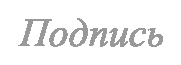
\includegraphics[width=3cm]{sec-facsimile}\hfill
\fi%
\makeatother%
\emph{В. Д. Скарин}

\clearpage

\normalsize
\nsection{1. Общая характеристика работы}

% Актуальность работы
\actualitysection
\actualitytext

	%Теорию решения некорректных задач развивали А.~Н.~Тихонов, М.~М.~Лаврентьев, В.~К.~Иванов, А.~Б.~Бакушинский, Б.~Т.~Поляк, А.~В.~Гончарский, В.~В.~Васин, А.~Л.~Агеев, В.~П.~Танана, А.~Г.~Ягола, A.~Neubauer, O.~Scherzer, B.~Kaltenbacher, U.~Tautenhahn и др.
	
	%Для решения систем нелинейных уравнений проводились исследования в работах Л.~В.~Канторовича, А.~Б.~Бакушинского, М.~Ю.~Кокуриным, Б.~Т.~Поляка, J.~M.~Ortega и W.~C.~Rheinboldt,	A.~Neubauer, M.~J.~D.~Powell, 	J.~C.~Gilbert, J.~Nocedal, S.~J.~Wright.
	%L.~Landweber, M.~Hanke. %Градиентные методы с применением метода Ландвебера исследовались М.~Ю.~Кокуриным.
	%Методы решения структурных обратных задач гравиметрии и магнитометрии предложены в работах В.~Б.~Гласко, В.~Н.~Страхова.
	
	Основы теории некорректно поставленных задач были заложены в 50--60 годы прошлого века в работах выдающихся российских математиков А.~Н.~Тихонова, В.~К.~Иванова, М.~М.~Лаврентьева и дальнейшее ее развитие было продолжено в работах их учеников и последователей. В этих работах исследования относились, главным образом, к линейным уравнениям, но и для нелинейных задач были сформулированы базовые принципы регуляризации.
	
	В последние три десятилетия получили развитие устойчивые (регулярные) методы решения нелинейных некорректных задач на основе принципа итеративной регуляризации и иных подходах. Эти исследования связаны с именами А.~Б.~Бакушинского, Б.~Т.~Поляка, А.~В.~Гончарского, М.~Ю.~Кокурина, В.~В.~Васина, В.~Г.~Романова, С.~И.~Кабанихина, Ф.~П.~Васильева, В.~А.~Морозова, А.~Г.~Яголы, А.~С.~Леонова, А.~Л.~Агеева, В.~П.~Тананы, В.~И.~Максимова, А.~И.~Короткого, А.~Б.~Смирновой, A.~Neubauer, B.Kaltenbacher, H.~W.~Engl, M.~Hanke, C.~Boeckmann.
	
	Структурные задачи гравиметрии и магнитометрии --- важный класс нелинейных некорректных задач. Если исходные данные о геофизических полях измеряются на большой площади, то это приводит к необходимости решать системы нелинейных уравнений большой размерности с использованием многопроцессорных вычислителей и технологий распараллеливания. Для их решения широко использовались регуляризованные методы Ньютона, Левенберга --Марквардта и процессы градиентного типа (А.~Б.~Бакушинский, М.~Ю.~Кокурин, В.~В.~Васин$^1$, Е.~Н.~Акимова$^2$, Л.~Ю.~Тимерханова, Г.~Я.~Пересторонина, В.~Е.~Мисилов), а также экономичный метод локальных поправок (П.~С.~Мартышко, И.~Л.~Пруткин$^3$).
	
	%Алгоритмы решения обратных задач математической физики на основе регуляризованных методов Ньютона, Левенберга -- Марквардта и градиентных методов разрабатывались в ИММ УрО РАН В.~В.~Васиным$^1$, Е.~Н.~Акимовой$^2$, 
	%Л.~Ю.~Тимерхановой, Г.~Я.~Пересторониной, В.~Е.~Мисиловым.
	{\scriptsize
	\let\thefootnote\relax\let\thefootnote\relax\footnotetext{\footnotesize 1. В. В. Васин, Г. Я. Пересторонина, И. Л. Пруткин, Л. Ю. Тимерханова. Решение трехмерных обратных задач гравиметрии и магнитометрии для трехслойной среды // Мат. мод. 2003. Т. 15, №2. С. 69--76.}
	\let\thefootnote\relax\let\thefootnote\relax\footnotetext{\footnotesize 2. Е. Н. Акимова. Параллельные алгоритмы решения обратных задач гравиметрии и магнитометрии на МВС-1000 // Вестник ННГУ. 2009. №4. С. 181--189.}
	%\let\thefootnote\relax\let\thefootnote\relax\footnotetext{\footnotesize 2. Akimova E. N., Vasin V. V. Stable Parallel algorythms for solving the inverse gravimetry and magnetometry problems // Intern. J. Engineering Modelling. 2004. Vol. 17. № 1-2, P. 13--19.}
	\let\thefootnote\relax\let\thefootnote\relax\footnotetext{\footnotesize 3. И. Л. Пруткин. О решении трехмерной обратной задачи гравиметрии в классе контактных поверхностей методом локальных поправок // Изв. АН СССР. Физика Земли. 1986. №1. С. 67--77.}
	%\let\thefootnote\relax\let\thefootnote\relax\footnotetext{\footnotesize 3. П. С. Мартышко, И. В. Ладовский, А. Г. Цидаев. Построение региональных геофизических моделей на основе комплексной интерпретации гравитационных и сейсмических данных // Физика Земли. 2010. №11. С. 23--35.}	
	} 
	
%	Алгоритмы решения геофизических задач на основе метода локальных поправок разрабатывались в ИГФ УрО РАН 
%	П.~С.~Мартышко$^3$, И.~Л.~Пруткиным. 
%	{\scriptsize
%	\let\thefootnote\relax\let\thefootnote\relax\footnotetext{\footnotesize 4. П. С. Мартышко, И. В. Ладовский, А. Г. Цидаев. Построение региональных геофизических моделей на основе комплексной интерпретации гравитационных и сейсмических данных // Физика Земли. 2010. №11. С. 23--35.}
%	}

% Степень разработанности темы исследования
%\developmentsection
%\developmenttext

% Цели и задачи диссертационной работы
\objectivesection
\objectivetext

% Методология и методы исследования
\methodssection
\methodstext

% Научная новизна
\noveltysection
\noveltytext

% Теоретическая и практическая значимость
\valuesection
\valuetext

% Положения, выносимые на защиту
%\resultssection
%\resultstext

% Степень достоверности и апробация результатов
\approbationsection
\approbationtext

% Публикации
\pubsection
\pubtext

% Личный вклад автора
\contribsection
\contribtext

% Структура и объем диссертации
\structsection
\structtext

Исследования по теме диссертации выполнены в период с 2013 по 2017 годы в Отделе некорректных задач анализа и приложений Института математики и махеники УрО РАН.

Автор выражает искреннюю признательность своему научному руководителю доктору физико-математических наук, ведущему научному сотруднику ИММ УрО РАН Елене Николаевне Акимовой.

Автор выражает благодарность за постановку ряда проблем, поддержку, полезные замечания и обсуждения член-корреспонденту РАН, главному научному сотруднику ИММ УрО РАН Владимиру Васильевичу Васину.

\nsection{2. Содержание работы}

Во \textbf{введении} обосновывается актуальность темы исследований и выполнен краткий обзор публикаций по теме диссертации, сформулирована цель работы, показаны научная новизна и практическая значимость полученных результатов.

\textbf{В первой главе} рассматриваются методы решения некорректных задач с монотонным оператором. Обоснован двухэтапный метод на основе  регуляризованного метода Ньютона. Построены методы минимальной ошибки, наискорейшего спуска и минимальных невязок решения нелинейных уравнений и доказывается их сходимость к регуляризованному решению.

Рассматривается нелинейное уравнение $I$ рода
\begin{equation}\label{equ1}A(u)=f\end{equation}
в гильбертовом пространстве с монотонным непрерывно дифференцируемым по Фреше оператором $A$, для которого обратные операторы $A'(u)^{-1}$, $A^{-1}$ разрывны в окрестности решения, что влечет некорректность задачи $\eqref{equ1}$. Для построения регуляризующего алгоритма используется двухэтапный метод, в котором на первом этапе используется регуляризация по схеме Лаврентьева
\begin{equation}\label{equ2}A(u)+\alpha(u-u^0)-f_\delta=0,\end{equation}
где $\|f-f_\delta\|\leqslant\delta$, $u_0$ --- некоторое приближение к решению; а на втором этапе для аппроксимации регуляризованного решения $u_\alpha$ применяется либо регуляризованный метод Ньютона (РМН) (А. Б. Бакушинский$^{4,5}$ ($\gamma=1$, $\bar{\alpha}=\alpha=\alpha_k$)):
\vskip -10 mm
%либо модифицированный регуляризованный метод Ньютона,
{\scriptsize
	\let\thefootnote\relax\let\thefootnote\relax\footnotetext{\footnotesize 4. А. Б. Бакушинский. Регуляризующий алгоритм на основе метода Ньютона -- Канторовича для решения вариационных неравенств // ЖВМиМФ, 16:6 (1976). С. 1397--1604.}
	\let\thefootnote\relax\let\thefootnote\relax\footnotetext{ 5. A. Bakushinsky, A. Goncharsky. Ill-Posed Problems: Theory and Applications. Berlin; Boston; London: Kluwer Academic Publishers, 1994. 258~p.}
	%\let\thefootnote\relax\let\thefootnote\relax\footnotetext{\footnotesize 5. В. В. Васин, Е. Н. Акимова, А. Ф. Миниахметова. Итерационные алгоритмы ньютоновского типа и их приложения к обратной задаче гравиметрии // Вестник ЮУрГУ, 6:3 (2013). С. 26--37.}
}
\begin{equation}\label{equ_rmn}
u^{k+1}=u^k-\gamma(A'(u^k)+\bar\alpha I)^{-1}(A(u^k)+\alpha(u^k-u^0)-f_\delta)\equiv{T(u^k)},
\end{equation}
либо нелинейные аналоги $\alpha$-процессов
\begin{equation}\label{equ_alphaproc}
u^{k+1}=u^k-\gamma\frac{\langle (A'(u^k)+\bar\alpha I)^{\varkappa}S_\alpha(u^k), S_\alpha(u^k)\rangle }{\langle(A'(u^k)+\bar\alpha I)^{\varkappa+1}S_\alpha(u^k), S_\alpha(u^k)\rangle }S_\alpha(u^k)\equiv{T(u^k)}
\end{equation}
при $\varkappa=-1,0,1$. Здесь $\alpha>0, \bar\alpha>0$ --- параметры регуляризации, $\gamma>0$ --- демпфирующий множитель, $S_\alpha(u)=A(u)+\alpha(u-u^0)-f_\delta$.
\begin{remark}
	Формула $\eqref{equ_alphaproc}$ при $\varkappa=1$ справедлива лишь для самосопряженного оператора $A'(u)$. В общем случае, знаменатель дроби при $\varkappa=1$ следует заменить на $\|(A'(u)+\alpha I)S_\alpha (u)\|^2$.
\end{remark}

Впервые итерационные $\alpha$-процессы были предложены в работах М.~А.~Крас\-носельского$^6$ и др. для решения линейного уравнения с ограниченным, самосопряженным, положительно определенным оператором. Для линейных некорректных операторных уравнений итеративно регуляризованные $\alpha$-процессы были исследованы в монографии$^5$. Нелинейные аналоги модифицированных $\alpha$-про\-цессов были предложены и изучены в работе В.~В.~Васина$^7$.

{\scriptsize
	\let\thefootnote\relax\let\thefootnote\relax\footnotetext{\footnotesize 6. М. А. Красносельский, Г. М. Забрейко, П. П. Забрейко и др. Приближенное решение операторных уравнений // М.: Наука, 1969.}
	\let\thefootnote\relax\let\thefootnote\relax\footnotetext{\footnotesize 7. В. В. Васин. Регуляризованные модифицированные $\alpha$-процессы для нелинейных уравнений с монотонным оператором // ДАН. 2016. Т.94, №1. С.13--16.}
}

Так как оператор $A$ --- монотонный, то его производная $A'(u^k)$ --- неотрицательно определенный оператор. Операторы $(A'(u^k)+\bar\alpha I)^{-1}$ существуют и ограничены, следовательно, процессы $\eqref{equ_rmn}$, $\eqref{equ_alphaproc}$ определены корректно.
%Итеративно регуляризованный метод Ньютона ($\gamma=1$, $ \bar\alpha=\alpha={\alpha}_k$) для вариационных неравенств был предложен и исследован ранее в работах А. Б. Бакушинского, А. В. Гончарского, где априори выбирается последовательность ${\alpha}_{k(\delta)}$ и при некоторых условиях, в том числе на вторую производную оператора $A$, доказывается сходимость итераций к решению уравнения $\eqref{equ1}$. 

В данной главе в предположении, что производная $A'(u)$ удовлетворяет условию Липшица, устанавливается линейная скорость сходимости методов $\eqref{equ_rmn}$,  $\eqref{equ_alphaproc}$ и свойство фейеровости итераций. При истокообразной представимости решения асимптотическое правило останова итераций $k(\delta)$ определяется из равенства оценок погрешности для итераций и регуляризованного решения $u_\alpha$.

Пусть имеются следующие условия
\begin{equation}\label{cond1.1}
\|A(u)-A(v)\|\leqslant N_1\|u-v\|, \quad
\|A'(u)-A'(v)\|\leqslant N_2\|u-v\|, \quad \forall u, v \in S_r(u^0).
\end{equation}
и известна оценка для нормы производной в точке $u^0$ (начальном приближении), т.е.
\begin{equation}\label{cond1.3}
\|A'(u^0)\| \leqslant N_0\leqslant N_1, \quad \|u^0-u_\alpha\| \leqslant r.
\end{equation}

\begin{theorem}\label{teo2.1} Пусть $A$ --- монотонный оператор, для которого выполнены условия $\eqref{cond1.1}$ для $u, v \in S_r(u_\alpha)$, $r\leqslant \alpha/N_2$, $0<\alpha \leqslant \bar\alpha$, $\|u^0-u_\alpha\| \leqslant r$. 
	
	Тогда для процесса $\eqref{equ_rmn}$ c $\gamma=1$ имеет место линейная скорость сходимости метода при аппроксимации единственного решения $u_\alpha$ регуляризованного уравнения $\eqref{equ2}$
	\begin{equation}\label{nwt_conv}
	\| u^k-u_\alpha \| \leqslant q^kr, \quad q=(1-\frac{\alpha}{2\bar\alpha}).
	\end{equation}
\end{theorem}

Усиленное свойство Фейера$^8$ для оператора $T$ означает, что для некоторого $\nu>0$ выполнено соотношение
\begin{equation}\label{fejer_prop_uni}
{\|T(u)-z\|}^2\leqslant{\|u-z\|}^2-\nu{\|u-T(u)\|}^2,
\end{equation}
где $z\in Fix(T)$ --- множество неподвижных точек оператора $T$. Это влечет для итерационных точек $u^k$, порождаемых процессом $u^{k+1}=T(u^k)$, выполнение неравенства
\begin{equation}\label{fejer_prop_it}
{\|u^{k+1}-z\|}^2\leqslant{\|u^k-z\|}^2-\nu{\|u^k-u^{k+1}\|}^2.
\end{equation}
{\scriptsize
\let\thefootnote\relax\let\thefootnote\relax\footnotetext{\footnotesize 8. В. В. Васин, И. И. Еремин. Операторы и итерационные процессы фейеровского типа. Теория и приложения. Екатеринбург: УрО РАН, 2005.}}
Важным свойством фейеровских операторов является замкнутость относительно операций произведения и взятия выпуклой суммы. Итерационные процессы с фейеровским оператором шага и общим множеством неподвижных точек позволяют строить гибридные методы, а также учитывать априорные ограничения на решение в виде систем неравенств.

\begin{theorem} \label{teo2.3}
	Пусть выполнены условия $\eqref{cond1.1}$--$\eqref{cond1.3}$, $A'(u^0)$ --- самосопряженный оператор, $\|u_\alpha-u^0\|\leqslant r$, 
$0\leqslant\alpha\leqslant\bar\alpha$, $\bar\alpha\geqslant 4N_1$, $r\leqslant\alpha/8N_2$. Тогда при
	$\gamma<\frac{\alpha\bar\alpha}{2(N_1+\alpha)^2}$
	оператор шага $T$ процесса $\eqref{equ_rmn}$ при
	$$\nu=\frac{\alpha\bar\alpha}{2\gamma(N_1+\alpha)^2}-1$$
	удовлетворяет неравенству $\eqref{fejer_prop_uni}$, для итераций $u^k$ справедливо соотношение $\eqref{fejer_prop_it}$ и имеет место сходимость
	$\lim_{k\to\infty}\|u^k-u_\alpha\|=0.$
	Если параметр $\gamma$ принимает значение ${\gamma}_{opt}=\frac{\alpha\bar\alpha}{4(N_1+\alpha)^2},$ то справедлива оценка $$\|u^k-u_\alpha\|\leqslant q^k r, \quad q=\sqrt{1-\frac{{\alpha}^2}  {16(N_1+\alpha)^2}}.$$
\end{theorem}

Далее приводится оценка скорости сходимости нелинейных $\alpha$-процессов.
\begin{theorem}\label{teo3.2}
	Пусть выполнены условия $\eqref{cond1.1}$--$\eqref{cond1.3}$, $A'(u^0)$ --- самосопряженный оператор, для ММО $\alpha \leqslant \bar\alpha$,  $r\leqslant \alpha/8N_2$, $\bar\alpha \geqslant N_0$.  Тогда при
	$$\gamma _\varkappa <\frac{2}{\mu _\varkappa}\quad (\varkappa=-1,0,1)$$
	для последовательности $\{u^k\}$, порождаемой $\alpha$-процессом при соответствующем $\mu_\varkappa$, имеет место сходимость $\lim_{k\to\infty}\|u^k-u_\alpha\|=0, $ а при 
	$\gamma{_\varkappa^{opt}}=\frac{1}{\mu_\varkappa}$
	справедлива оценка $\|u^k-u_\alpha\|\leqslant q{_\varkappa^k}r,$ где
	$$
	q_{-1}=\sqrt{1-\frac{\alpha^2}{16(N_1+\alpha)^2}}, \quad q_0=\sqrt{1-\frac{\alpha^2\bar\alpha^2}{(N_1+\alpha)^2(N_1+\bar\alpha)^2}}, \quad $$$$q_1=\sqrt{1-\frac{\alpha^2\bar\alpha^4}{(N_1+\bar\alpha)^4}}.
	$$
\end{theorem}

%Результаты первой главы опубликованы в работе~\cite{VasSkur2017,}.

\textbf{Во второй главе} обоснована сходимость к регуляризованному решению итераций РМН, ММО, МНС, ММН в~конечномерном случае без требования монотонности оператора $A$ исходного уравнения. Представлены результаты численных экспериментов.

Пусть собственные значения $\lambda _i$ матрицы $A'(u)$ $n\times n$ различны между собой и неотрицательны. Тогда при $\bar\alpha>0$ матрица имеет представление $A'(u)+\bar\alpha I =S(u)\Lambda S^{-1}(u)$ и справедлива оценка
\begin{equation}\label{est4.1}
\|(A'(u)+\bar\alpha I)^{-1}\|\leqslant \frac{\mu (S(u))}{\bar\alpha+\lambda_{min}} \leqslant \frac{\mu(S(u))}{\bar\alpha},
\end{equation}
где столбцы матрицы $S(u)$ составлены из собственных векторов матрицы $A'(u)+\bar\alpha I$, $\Lambda$ --- диагональная матрица, ее элементы --- собственные значения матрицы $A'(u)+\bar\alpha I$, $\mu(S(u))=\|S(u)\|\cdot\|S^{-1}(u)\|$.

Рассмотрим теперь вариант теорем 2, 3, когда оператор $A\colon R^n \to R^n$ и его производная имеет неотрицательный спектр. Имея оценку $\eqref{est4.1}$, доказывается теорема для регуляризованного метода Ньютона
\begin{theorem}\label{conv_rate_nemonot_nwt}
	Пусть выполнены условия $\eqref{cond1.1}$--$\eqref{cond1.3}$, а также: $\sup\{\mu(S(u)): u\in S_r(u_\alpha)\}\leqslant\bar S <\infty,$ 
	$A'(u^0)$ --- симметричная матрица, $0<\alpha\leqslant\bar\alpha$, $\bar\alpha\geqslant 4N_0$, $r\leqslant\alpha/8N_2\bar S$.

	Тогда для метода $\eqref{equ_rmn}$ справедливо заключение теоремы (1.3), где
	$$\gamma<\frac{\alpha\bar\alpha}{2(N_1+\alpha)^2\bar S^2},
	\quad
	{\gamma}_{opt}=\frac{\alpha\bar\alpha}{4(N_1+\alpha)^2\bar S^2},$$ 
	$$\|u^k-u_\alpha\|\leqslant q^k r, \quad q=\sqrt{1-\frac{\alpha ^2}{16(N_1+\alpha)^2\bar S^2}}.$$
\end{theorem}
Аналогично имеем теорему о сходимости ММО, МНС и ММН.
\begin{theorem}\label{conv_rate_nemonot_alpha}
Пусть выполнены условия теоремы 4. 
Тогда при $\gamma_\varkappa<2/\mu _\varkappa$, $\varkappa=-1,0,1$, с соответствующими $\mu _k$ для каждого процесса, последовательности ${u^k}$, порождаемые процессом $\eqref{equ_alphaproc}$ при $\varkappa=-1,0,1$, сходятся к $u_\alpha$, т.е., $\lim_{k\to\infty}\|u^k-u_\alpha\|=0,$ а при $
\gamma{_\varkappa^{opt}}=1/\mu_\varkappa$
справедлива оценка $\|u^{k+1}-u_\alpha\|\leqslant q{_\varkappa^k}r,$ где
$$q_{-1}=\sqrt{1-\frac{\alpha^2}{64\bar S^2(N_1+\alpha)^2}}, \quad q_0=\sqrt{1-\frac{\alpha^2\bar\alpha^2}{36(N_1+\alpha)^2(N_1+\bar\alpha)^2}},$$
$$q_1=\sqrt{1-\frac{\alpha^2\bar\alpha^6}{36(N_1+\alpha)^2(N_1+\bar\alpha)^6}}.$$
\end{theorem}
Для модифицированных ММО, МНС и ММН, где производная $A'(u)$ вычисляется в фиксированной точке $u^0$, также обосновывается сходимость.	
\begin{theorem}\label{conv_rate_nemonot_alpha_mod}
	Пусть выполнены условия $\eqref{cond1.1}$--$\eqref{cond1.3}$ $A'(u^0)$ --- самосопряженный оператор, спектр которого состоит из неотрицательных различных собственных значений, 
	$0\leqslant\alpha\leqslant\bar{\alpha}, \quad r=\alpha/6N_2, \quad \bar{\alpha}\geqslant N_0$. Тогда при
	$\gamma _\varkappa <2/\mu _\varkappa \quad (\varkappa=-1,0,1)$
	для последовательности $\{u^k\}$, порождаемой модифицированным $\alpha$-процессом при соответствующем $\varkappa$, имеет место сходимость $\lim_{k\to\infty}\|u^k-u_\alpha\|=0, $ а при 
	$\gamma{_\varkappa^{opt}}=\frac{1}{\mu_\varkappa}$
	справедлива оценка $\|u^k-u_\alpha\|\leqslant q{_\varkappa^k}r,$ где
	$q^\varkappa=\sqrt{1-\frac{9\alpha^2}{64(N_1+\alpha)^2}}$.
\end{theorem}
\begin{remark}
	Предложенный подход к получению оценок скорости сходимости итерационных процессов полностью переносится на случай, когда спектр матрицы $A'(u^k)$, состоящий из различных вещественных значений, содержит набор малых по абсолютной величине отрицательных собственных значений. Пусть $\lambda _1$ --- отрицательное собственное значение с наименьшим модулем $|\lambda_1|$ и $\bar\alpha -|\lambda _1|=\bar\alpha _1<\alpha^*$. Тогда оценка $\eqref{est4.1}$ 
	трансформируется в неравенство
	$$\|(A'(u^k)+\bar\alpha I)^{-1}\|\leqslant\frac{\mu(S(u^k))}{\bar\alpha^*}\leqslant\frac{\bar S}{\bar\alpha^*}.$$
	Все теоремы остаются справедливыми при замене $\bar\alpha$ на $\bar\alpha^*$.
\end{remark}

В работе$^9$ (теорема 5.1.) приводится оптимальная по порядку оценка погрешности двухэтапного метода с монотонным оператором:
\begin{equation*}
\|u_{\alpha(\delta)}^{\delta, k}-\hat{u}\|\leqslant 4\sqrt{k_0 \delta},
\end{equation*}
где $u_{\alpha(\delta)}^{\delta, k}$ --- $k$-е приближение, $\hat{u}$ --- решение уравнения (\ref{equ1}), $k_0=(1+N_2\|v\|/2)\|v\|$ ($u^0-\hat{u}=A'(\hat{u})v$ --- истокообразная представимость решения). Для получения оценки используется результат U. Tautenhahn$^{10}$ для регуляризованного решения.
В конечномерном случае для оператора $A'(u)$ с положительным спектром установлена оценка для невязки --- основной характеристики точности метода при решении задачи с реальными данными.
$$\|A(u_{\alpha(\delta)}^{\delta,k})-f_\delta\|\leqslant 2m\delta^p,$$
где для $\alpha(\delta)$ ограничена величина $\|u_{\alpha(\delta)}^{\delta}-u^0\|\leqslant m <\infty$, $\alpha(\delta)=\delta^p$. 
{\scriptsize
\let\thefootnote\relax\let\thefootnote\relax\footnotetext{\footnotesize 9. В. В. Васин, А. Ф. Скурыдина. Двухэтапный метод построения регуляризующих алгоритмов для нелинейных некорректных задач // Труды ИММ УрО РАН. Т.23 В.1 (2017), С. 57–74.}
\let\thefootnote\relax\let\thefootnote\relax\footnotetext{\footnotesize 10. U. Tautenhahn. On the method of Lavrentiev regurarization for nonlinear ill-posed problems // Inverse Problem. 2002. Vol. 91, №1. P. 191–207.}
}

 Методы РМН, ММО, МНС, ММН и их модифицированные варианты использованы при решении обратной структурной задачи магнитометрии
\begin{equation*}\begin{aligned}
\left[A(u)\right](x,y)=\frac{\mu_0}{4\pi}\Delta J  \bigg\{&\iint_{D} \frac{H}{[(x-x')^2+(y-y')^2+H^2]^{3/2}}dx'dy' \notag\\
- &\iint_{D} \frac{u(x',y')}{[(x-x')^2+(y-y')^2+u^2(x',y')]^{3/2}}dx'dy' \bigg\}= B_z(x,y,0),
\end{aligned} \end{equation*}
где $\mu_0/{4\pi}=10^{-7}$ Гн/м --- магнитная постоянная, $\Delta J$ --- скачок $z$-компоненты вектора намагниченности, $z=H$ --- асимптотическая плоскость, $ B_z(x,y,0)$ --- функция, описывающая  аномальное поле, $D=\{c\leqslant x' \leqslant d, a\leqslant y' \leqslant b\}$, $z=u(x,y)$ --- искомая функция.

Число обусловленности $\mu(A'_n(u_n^k))\approx 1.8\cdot 10^7$, спектр является неотрицательным и состоит из различных собственных значений, $\bar\alpha=10^{-2}$, $\alpha = 10^{-4}$, $\gamma=1$, $\varepsilon =\|u^k-z\|/\|z\| < 10^{-2}$. Итерационные методы достигают точности $\varepsilon$ за 4--5 итераций, у модифицированных методов меньше время счета.

%Результаты второй главы опубликованы в работах~\cite{VasSkur2017,VasSkur2015}.

\textbf{В третьей главе} предложены покомпонентные методы типа Ньютона и типа Левенберга -- Марквардта, а также вычислительная оптимизация методов типа Ньютона. Параллельные алгоритмы реализованы в виде комплекса программ на многоядерных и графических процессорах.

1. Задача гравиметрии о нахождении поверхности раздела в декартовой системе координат с осью $z$, направленной вниз, имеет вид
\vskip -2 mm
\begin{equation}\label{equ_grav_2l}
\begin{aligned}
A(u)=f\Delta\sigma \bigg\{ &\iint_{D} \frac{1}{[(x-x')^2+(y-y')^2+H^2]^{1/2}}dx'dy' \\
- &\iint_{D} \frac{1}{[(x-x')^2+(y-y')^2+u^2(x',y')]^{1/2}}dx'dy'\bigg\}=\Delta g(x,y,0),
\end{aligned} 
\end{equation}
	где $f$ --- гравитационная постоянная, равная $6.67\cdot10^{-8}$ см$^3/$г$\cdot c^2$, $\Delta\sigma=\sigma_2-\sigma_1$ --- скачок плотности на поверхности раздела сред $u(x,y)$, $D=\{c\leqslant x \leqslant d, a\leqslant y \leqslant b\}$, $\Delta g(x,y,0)$ --- аномальное гравитационное поле.%, вызванное отклонением поверхности от асимптотической плоскости $z=H$ для искомого решения $u(x,y)$.
	
	Итерации в методе Ньютона строятся по схеме
$$A'(u^k)(\Delta u^k)=-\big[A(u^k)-f\big],$$ где $A(u)=\int_{a}^{b}\int_{c}^{d}K(x,y, x',y',u^k(x,y))dxdy$ --- интегральный оператор задачи гравиметрии, $\Delta u^k=u^{k+1}-u^k$.
Т.е., для задачи гравиметрии
\begin{equation}\label{newton_integral_equ}
	f\Delta\sigma\int_{a}^{b}\int_{c}^{d}K'_u(x,y, x',y',u^k(x,y))\Delta u^k(x,y) dxdy=-\big[A(u(x',y'))-f(x',y')\big].
\end{equation}

%\begin{remark} (И. Л. Пруткин)
%	На значение гравитационного поля в точке $(x',y')$ наибольшее влияние оказывает глубина залегания поверхности в точке.
%\end{remark}  
Полагая $\Delta u^k(x,y)=\Delta u^k(x',y')=const$ относительно переменных интегрирования, перейдем от $\eqref{newton_integral_equ}$ к приближенному соотношению
$$f\Delta\sigma(\Delta u^k(x',y'))\int_{a}^{b}\int_{c}^{d}K'_u(x,y, x',y',u^k(x,y)) dxdy\approx A(u(x',y'))-f(x',y').$$

%Регуляризованный метод Ньютона имеет вид$^4$:
%$$ u^{k+1}=u^k-\gamma(A'(u^k)+\bar\alpha I)^{-1}(A(u^k)+\alpha(u^k-u^0)-f_\delta).$$

Покомпонентный метод типа Ньютона имеет вид$^{11}$:
$$u^{k+1}(x',y')=u^k(x',y')-\gamma\frac{1}{\varPsi(x',y')}\big([A(u^k)](x',y')-f(x',y')\big),$$
где $\varPsi(x',y')=f\Delta\sigma\int_{a}^{b}\int_{c}^{d}K'_u(x,y, x',y',u^k(x,y)) dxdy.$

Регуляризованный покомпонентный метод типа Ньютона имеет вид:
$$u^{k+1}(x',y')=u^k(x',y')-\gamma\frac{1}{\varPsi(x',y')+\bar{\alpha}}([A(u^k)](x',y')+$$ 
$$+\alpha (u^k(x',y')-u^0(x',y'))-f_\delta(x',y')),$$
где $\gamma$ --- демпфирующий множитель, $\alpha, \bar{\alpha}$ --- положительные параметры регуляризации.

В дискретной записи итерационный процесс запишется
$$u_{m,l}^{k+1}=u_{m,l}^k-\frac{1}{\psi_{m,l}^k+\bar\alpha}([A_n(u^k)]_{m,l} + \alpha(u^k-u^0) -f_{m,l}),\quad 1\le m \le M, \quad 1\le l \le N,$$
{\scriptsize
	\let\thefootnote\relax\let\thefootnote\relax\footnotetext{\footnotesize 11. Akimova E., Skurydina A. A componentwise Newton type method for solving the structural inverse gravity problem // EAGE Geoinformatics 2015}
}
где $\psi_{m,l}^k=f\Delta\sigma\sum\limits_{i=1}^{M}\sum\limits_{j=1}^{N}
\Delta x\Delta y\frac{u_{ij}}{[(x_k-x'_j)^2+(y_l-y'_i)^2+(u_{ij})^2]^{3/2}}$, $n=M\cdot N$.
Сумма $\psi_{m,l}^k$ --- сумма элементов $(m\times M + l)$-й строки матрицы производной $A'_n(u_n^k)$.
Вычислительная сложность покомпонентного метода типа Ньютона для решения системы $n$ уравнений без учета сложности алгоритма вычисления $A_n(u_n^k)$ составляет $O(n)$, в отличие от метода Ньютона, где сложность алгоритма $O(n^2)$.

2. Предложена вычислительная оптимизация метода Ньютона. Прозводная оператора $A$ в точке $u^k(x,y)$ определяется формулой:
\begin{itemize}
	\item в задаче гравиметрии
	$$ [A'(u)]h=\iint_{D} \frac{u^k(x',y')h(x',y')}{[(x-x')^2+(y-y')^2+(u^k(x',y'))^2]^{3/2}}dx'dy',$$
	\item в задаче магнитометрии
	$$ [A'(u^k)]h=\iint_{D} \frac{(x-x')^2+(y-y')^2-2(u^k(x',y'))^2}{[(x-x')^2+(y-y')^2+(u^k(x',y'))^2]^{5/2}}h(x',y')dx'dy'.$$
\end{itemize}
После дискретизации интегрального оператора и его производной, получаем матрицу $A'_n(u^k)$ с диагональным преобладанием$^{12}$.
Без существенной потери точности учитываются только значения элементов $a_{ij}$, где $i+j\in[i-\beta;i+\beta]$.
{\scriptsize
	\let\thefootnote\relax\let\thefootnote\relax\footnotetext{\footnotesize 12. Акимова Е. Н., Миниахметова А. Ф., Мартышко М. П. Оптимизация и распараллеливание методов типа  Ньютона для решения структурных обратных задач гравиметрии и магнитометрии // EAGE Geoinformatics 2014.}
	}
%Без существенной потери точности можно не учитывать значения элементов
%$a_{ij}$, где $j\notin[(i*n+i)-\beta;(i*n+i)+\beta]$.
%Без существенной потери точности можно не учитывать значения элементов, отстоящих от диагонали далее, чем на  $\beta$-ю часть  размерности матрицы производной., то есть те значения $a_{ij}$, для которых  $j \in \{i-h(\beta),..i+h(\beta)\} $, где $h(\beta)$ --- полуширина ленты матрицы, $i, j$ --- индекс элемента.

3. Задача гравиметрии о нахождении нескольких поверхностей раздела имеет вид (суммарное поле получаем сложением полей от каждой поверхности)
\begin{equation}\label{equ_grav_multi}
		\begin{aligned}
		& A(u)=\sum_{l=1}^{L}f\Delta\sigma_l\frac{1}{4\pi}\times 
		\iint_D\bigg\{\frac{1}{[(x-x')^2+(y-y')^2+u_l^2(x,y)]^{1/2}} \\
		&-\frac{1}{[(x-x')^2+(y-y')^2+H_l^2]^{1/2}}\bigg\}=\Delta g(x',y'),
		\end{aligned}
\end{equation}		
где $L$~--- число границ раздела, $f=6.67\cdot10^{-8}$ см$^3/$г$\cdot c^2$, $\Delta\sigma=\sigma_2-\sigma_1$ --- скачок плотности на поверхности раздела сред $u(x,y)$, $\Delta g(x,y,0)$ --- аномальное гравитационное поле.

Регуляризованный метод Левенберга -- Марквардта имеет вид 
$$u^{k+1}=u^k-\gamma[A'(u^k)^*A'(u^k)+\alpha I]^{-1} [A'(u^k)^*(A(u^k)-f_\delta)].$$

По аналогии с ПМН, запишем покомпонентный метод типа Левенберга -- Марквардта$^{13}$:
$$ u_l^{k+1}=u_l^k-\gamma\frac{1}{\varphi_l+\bar{\alpha}}\Lambda[ A'(u_l^k)^T(A(u^k)-f_\delta)],$$
где $l$ --- номер границы раздела, $l=1,..,L$, $\Lambda$ --- диагональный весовой оператор, 
%\begin{equation*}
%\begin{aligned}
%\varphi_l=\bigg[ f\Delta\sigma\int_{a}^{b}\int_{c}^{d}
%K'_u(x, y, x', y', u_l^k(x',y'))dxdy\bigg] \notag \\ \times\bigg[f\Delta\sigma\int_{a}^{b}\int_{c}^{d}K'_u(x,y, x',y',u_l^k(x,y))dxdy\bigg], 
%\end{aligned}
%\end{equation*} 
$\varphi_l=\bigg[ f\Delta\sigma\int_{a}^{b}\int_{c}^{d}
K'_u(x, y, x', y', u_l^k(x',y'))dxdy\bigg] \notag \\ \times\bigg[f\Delta\sigma\int_{a}^{b}\int_{c}^{d}K'_u(x,y, x',y',u_l^k(x,y))dxdy\bigg], $
где $K'_u(x',y', x, y, u_l^k(x',y'))$ --- ядро интегрального оператора. %транспонированного к ядру $K'_u(x,y,$ $ x',y',u^k(x,y))$.
% Величина $\varphi_l$ зависит от $u_l^k$.
{\scriptsize
\let\thefootnote\relax\let\thefootnote\relax\footnotetext{ 13. Skurydina A. F. Regularized Levenberg –- Marquardt Type Method Applied to the Structural Inverse Gravity Problem in a Multilayer Medium and its Parallel Realization // Bulletin of South Ural State University. 2017. V.6, N.3. pp. 5--15}}
В дискретной форме
\begin{equation*}\label{comp_lm_meth_disc}
u_{l,i}^{k+1}=u_{l,i}^k-\gamma\frac{1}{\varphi_{l,i}+\bar{\alpha}}w_{l,i}\bigg[ \{A'(u_l^k)^T(A(u^k)-f_\delta)\}_i\bigg],
\end{equation*}
где $w_{l,i}$ --- $i$-й весовой множитель, зависящий от $l$-й границы раздела,
\begin{equation*}
\begin{aligned}
\varphi_{l,i}=\bigg[ f\Delta\sigma\sum\limits_{k=1}^{N}
\sum\limits_{m=1}^{M}
K'_u(x'_k,y'_m, \{x, y\}_i, u_{l,i}^k) \Delta x' \Delta y'\bigg] \notag \\ \times\bigg[f\Delta\sigma\sum\limits_{k=1}^{N}
\sum\limits_{m=1}^{M}K'_u(x_k,y_m, \{x',y'\}_i,u_l^k(x_k,y_m))\Delta x \Delta y\bigg]. 
\end{aligned}
\end{equation*}
{\scriptsize
\let\thefootnote\relax\let\thefootnote\relax\footnotetext{\footnotesize 14. Е. Н. Акимова, В. Е. Мисилов, А. Ф. Скурыдина, А. И. Третьяков. Градиентные методы решения структурных обратных задач гравиметрии и магнитометрии на суперкомпьютере “Уран” // Вычислительные методы и программирование, 2015. Т. 16, 155–164.}}
Весовые множители выбираются по формулам из работы$^{14}$. 

По сравнению с методом Левенберга -- Марквадта, где вычислительная сложность алгоритмов достигает $O(n^3)$ в силу умножения матриц $[A'(u^k)^T A'(u^k)]$ и обращения матрицы $[A'(u^k)^T A'(u^k)+\alpha I]$, вычислительная сложность покомпонентного метода типа Левенберга -- Марквадта составляет $O(n^2)$.

4. Параллельные алгоритмы реализованы в виде комплекса программ на многоядерных и графических процессорах NVIDIA (видеокартах) с помощью технологий OpenMP и CUDA для решения задач гравиметрии и магнитометрии на сетках большого размера. 
Результаты решения структурной обратной задачи гравиметрии на сетках размера $512\times 512$ и $1000\times 1000$ продемонстрировали, что покомпонентный метод типа Ньютона работает в три раза быстрее метода Ньютона, а покомпонентный метод типа Левенберга -- Марквардта --- в десять раз быстрее метода Левенберга -- Марквардта. Таким образом, предлагаемые автором покомпонентные методы являются экономичными по затратам оперативной памяти и по количеству вычислительных операций.

\nsection{3. Основные результаты диссертации}

1. Для нелинейного уравнения с монотонным оператором дано обоснование двухэтапного метода на основе регуляризованного метода Ньютона. 
Построены нелинейные аналоги $\alpha$-процессов:  регуляризованные методы градиентного типа для решения нелинейного уравнения с монотонным оператором: метод минимальной ошибки, метод наискорейшего спуска, метод минимальных невязок. Доказаны теоремы сходимости и сильная фейеровость итерационных процессов при аппроксимации регуляризованного решения. Для задачи с немонотонным оператором и неотрицательным спектром его производной, обоснована сходимость метода  Ньютона и нелинейных $\alpha$-процессов к регуляризованному решению.

2. Для решения нелинейных интегральных уравнений обратных задач гравиметрии предложены экономичные покомпонентные методы 
типа Ньютона и типа Левенберга – Марквардта. Предложена вычислительная оптимизация метода 
Ньютона для задач, где матрица производной имеет диагональное преобладание. 

3. Разработан комплекс параллельных программ для многоядерных и графических процессоров (видеокарт) решения обратных задач гравиметрии и магнитометрии на сетках большой размерности методами ньютоновского типа и покомпонентными методами. 
\vskip 5 mm
%В дальнейшей научной работе автора предполагается исследование на сходимость покомпонентных методов типа Ньютона и Левенберга -- Марквардта.
% ----------------------------------------------------------------

\begingroup
\let\clearpage\relax
\printbibheading[title={Основные публикации по теме диссертации}]
\vskip -6 mm
%Если не работает - коммент-анкоммент, все будет чики-чики
\printbibliography[
heading=subbibliography,
keyword=hac,
title={Статьи в изданиях из перечня ВАК, SCOPUS}
]
\endgroup

\printbibliography[
heading=subbibliography,
keyword=nohac,
title={Другие публикации}
]
%\printbibliography[notkeyword=own,title={Цитированная литература}]

% ----------------------------------------------------------------
% Выходные данные
%\clearpage
%\thispagestyle{empty}
%\normalfont\selectfont
%\vspace*{2cm}
%\begin{center}
%\textit{Научное издание}\\
%\vskip 5cm
%\makeatletter
%\@author
%\vskip 1.5cm
%\@title{} на тему:\\
%\@topic\\
%\makeatother
%\end{center}
%\vfill

%Подписано в печать ... Формат $60\times 90$/16. Тираж 100 экз. Заказ 256.
%\noindent
%Санкт-Петербургская издательская фирма <<Наука>> РАН.
%199034, Санкт-Петербург, Менделеевская линия, 1,
%\href{http://www.naukaspb.spb.ru}{http://www.naukaspb.spb.ru}

\end{document}
